\section{Electrokinetics}

\subsection{Sress tensor in the electrosymmetic model}

\subsubsection{Definitions}

The total free energy functional is a function of the composition $\phi$, the density of the ionic species $\rho_\alpha$,

\beq
{\cal F}[\phi,\{\rho_\alpha\}] = \int d{\bf r} \;F\left(\phi({\bf r}),\{\rho_\alpha({\bf r})\}\right). 
\eeq

The free energy density can be factorised into a contribution from the composition and an ionic contribution according to

\beqa
F&=&F^{mix} +F^{ion}\\
F^{mix}&=& \frac{1}{2} \,A \,\phi^2 + \frac{1}{4} \,B \,\phi^4+ \frac{1}{2} \kappa(\bm{\nabla}\phi)^2\\
F^{ion,ex}&=& \sum_{\alpha=\pm} \rho_\alpha \left(V^{solv}_\alpha-\mu_\alpha +\frac{z_\alpha e}{2}\Psi \right).
\eeqa

In the ionic contribution we have omitted the ideal gas contribution of the ions.
The solvation energy is given by

\beqa
V^{solv}_\alpha({\bf r})=\Delta\mu_\alpha\frac{1+\phi({\bf r})}{2}
\eeqa

It is convenient to define the total free energy without electric field $F_0$, i.e. with vanishing electric potential:  

\beqa
F_0&=&F^{mix} +F^{ion,ex}|_{\Psi=0}
\eeqa

The Poisson equation reads
\beqa
\bm{\nabla}\left(\varepsilon({\bf r})\bm{\nabla}\Psi({\bf r})\right)=-\sum_{\alpha=\pm} e \,z_\alpha \,\rho_\alpha ({\bf r})
\eeqa

whereas the electric field is given by

\beq
{\bm E}=-{\bm \nabla}\Psi.
\eeq

The permittivity depends on the composition $\phi$ via

\beqa
\varepsilon({\bf r})=\bar{\varepsilon} \,(1-\gamma\,\phi({\bf r}))
\eeqa

The electric displacement field 

\beq
{\bm D}({\bf r})=\varepsilon({\bf r}){\bm E}({\bf r})
\eeq

The 'co-energy' density 

\beq
\tilde{F}=F_0-\frac{\varepsilon}{2}\bm{E}^2
\eeq

has the meaning of a Legendre transform of the free energy density $F_0$.

\subsubsection{Electromechanical stress tensor}

The electromechanical stress tensor is generally defined as \cite{Landau-ED, Melcher}. 

\beqa
\sigma_{i j}=\varepsilon E_i E_j + \delta_{i j}\left( \tilde{F} - \phi \frac{\delta \tilde{\cal F}}{\delta\phi} - \sum_{\alpha=\pm} \rho_\alpha \frac{\delta \tilde{\cal F}}{\delta\rho_\alpha}\right).
\eeqa

The first functional derivative yields

\beqa
\phi \frac{\delta\tilde{\cal F}}{\delta\phi}&=&\phi\left(\frac{\delta {\cal F}_0}{\delta\phi}-\frac{{\bm E}^2}{2} \frac{\partial \varepsilon}{\partial\phi}\right)\\
&=&\phi\left(\frac{\partial F_0}{\partial\phi}-{\bm \nabla}\left(\frac{\partial F_0}{\partial {\bm \nabla}\phi}\right)-\frac{{\bm E}^2}{2} \frac{\partial \varepsilon}{\partial\phi}\right)\\
&=&A\,\phi^2+B\,\phi^4-\kappa\phi({\bm \nabla}^2\phi)+\frac{\phi}{2}\sum_{\alpha=\pm} \rho_\alpha \Delta\mu_\alpha+\phi\,\frac{\bar{\varepsilon}\gamma}{2}{\bm E}^2\\
&=&A\,\phi^2+B\,\phi^4-\kappa\phi({\bm \nabla}^2\phi)+\frac{\phi}{2}\sum_{\alpha=\pm} \rho_\alpha \Delta\mu_\alpha-\frac{\varepsilon-\bar{\varepsilon}}{2}{\bm E}^2,
\eeqa

where we used the above dependence of the permittivity on the composition.
The second functional derivative is given by 

\beqa
\rho_\alpha \frac{\delta \tilde{\cal F}}{\delta\rho_\alpha}&=&\rho_\alpha\left(\frac{\delta {\cal F}_0}{\delta\rho_\alpha}\right)\\
&=&\rho_\alpha(V^{solv}_\alpha-\mu_\alpha)
\eeqa

The co-energy density and the functional derivatives with respect to composition $\phi$ and ionic densities $\rho_\alpha$ add up to 

\beqa
\tilde{F} - \phi \frac{\delta \tilde{F}}{\delta\phi} - \sum_{\alpha=\pm} \rho_\alpha \frac{\delta \tilde{F}}{\delta\rho_\alpha}=&&\nonumber\\
&&\hspace*{-4cm}=-\frac{\varepsilon}{2}\bm{E}^2+\frac{A}{2} \phi^2 + \frac{B}{4} \phi^4+ \frac{\kappa}{2} (\bm{\nabla}\phi)^2 \nonumber\\
&&\hspace*{-3cm}-A\phi^2-B\phi^4+ \kappa\phi({\bm \nabla}^2\phi) -\frac{\phi}{2}\sum_{\alpha=\pm} \rho_\alpha \Delta\mu_\alpha\nonumber\\
&&\hspace*{-3cm}-\phi\,\frac{\bar{\varepsilon}\gamma}{2}{\bm E}^2-\sum_{\alpha=\pm}\rho_\alpha(V^{solv}_\alpha-\mu_\alpha)\\
&&\hspace*{-4cm}=-\frac{\varepsilon}{2}\bm{E}^2-\frac{A}{2}\phi^2 -\frac{3 B}{4} \phi^4+ \frac{\kappa}{2}(\bm{\nabla}\phi)^2 + \kappa\phi({\bm \nabla}^2\phi) \nonumber\\
&&\hspace*{-3cm}-\frac{\phi}{2}\sum_{\alpha=\pm} \rho_\alpha \Delta\mu_\alpha -\phi\,\frac{\bar{\varepsilon}\gamma}{2}{\bm E}^2
\eeqa

This yields

\beqa
\sigma_{ij}&=&\varepsilon E_i E_j - \delta_{i j}\left(\frac{\varepsilon}{2}\bm{E}^2+\frac{A}{2}\phi^2 +\frac{3\,B}{4}\phi^4 - \frac{\kappa}{2} (\bm{\nabla}\phi)^2\right.\nonumber\\
&&\left.- \kappa\phi({\bm \nabla}^2\phi) +\frac{\phi}{2}\sum_{\alpha=\pm} \rho_\alpha \Delta\mu_\alpha +\phi\,\frac{\bar{\varepsilon}\gamma}{2}{\bm E}^2\right).\nonumber\\
\eeqa

In order to satisfy the condition of mechanical equilibrium $\nabla_j \sigma_{ij}=0$ a symmetric contribution has to be added to the above stress tensor. The following lines try to elucidate this.\\

Taking the divergence of the stress tensor gives

\beqa
\nabla_j\sigma_{i j}&=& (\nabla_j \varepsilon E_j) E_i + \varepsilon E_j \nabla_j E_i + \nabla_i\left( \tilde{F} - \phi \frac{\delta \tilde{\cal F}}{\delta\phi} - \sum_{\alpha=\pm} \rho_\alpha \frac{\delta \tilde{\cal F}}{\delta\rho_\alpha}\right)\\
&=& \left({\bm \nabla}\cdot{\bm D}\right) E_i+ D_j \nabla_j E_i +\nabla_i F_0 - D_j \nabla_i E_j \nonumber\\
&&\hspace*{0.5cm} -\nabla_i\left(\phi \frac{\delta \tilde{\cal F}}{\delta\phi} +\sum_{\alpha=\pm} \rho_\alpha \frac{\delta \tilde{\cal F}}{\delta\rho_\alpha}\right)\\
&=& \left({\bm \nabla}\cdot{\bm D}\right) E_i + D_j \left(\nabla_j E_i-\nabla_i E_j\right) + \nabla_i F_0\nonumber\\
&&\hspace*{0.5cm} -\nabla_i\left(\phi \mu_\phi +\sum_{\alpha=\pm} \rho_\alpha \mu_{\rho_\alpha}\right)
\eeqa

According to Gauss' law the first term is 

\beq
\left({\bm \nabla}\cdot{\bm D}\right)E_i = \rho_f E_i=\sum_{\alpha=\pm} z_\alpha e \rho_\alpha E_i,
\eeq
 
whereas $\rho_f$ is the free charge density.
Moreover, due to Faraday's law the curl in the second bracket vanishes.
This leads us to the following intermediate result: 

\beqa
\nabla_j\sigma_{i j}&=& \sum_{\alpha=\pm}z_\alpha e \rho_\alpha E_i + \nabla_i F_0 - \nabla_i\left(\phi \mu_\phi +\sum_{\alpha=\pm} \rho_\alpha \mu_{\rho_\alpha}\right)\\
&=&\sum_{\alpha=\pm} z_\alpha e \rho_\alpha E_i + \frac{\partial F_0}{\partial \phi} \nabla_i \phi + \frac{\partial F_0}{\partial \nabla_j \phi} \nabla_j \nabla_i \phi +\sum_{\alpha=\pm} \left\{\frac{\partial F_0}{\partial \rho_\alpha}\right\} \nabla_i \rho_\alpha\nonumber\\
&&\hspace*{0.5cm} -\nabla_i\left(\phi \mu_\phi +\sum_{\alpha=\pm} \rho_\alpha \mu_{\rho_\alpha}\right)\\
&=& \sum_{\alpha=\pm} z_\alpha e \rho_\alpha E_i + \left\{\frac{\partial F_0}{\partial \phi} - \nabla_j \left(\frac{\partial F_0}{\partial \nabla_j \phi}\right)\right\} \nabla_i \phi +\nabla_j\left(\frac{\partial F_0}{\partial \nabla_j \phi} \nabla_i \phi\right)\nonumber\\
&&\hspace*{0.5cm} +\sum_{\alpha=\pm} \left\{\frac{\partial F_0}{\partial \rho_\alpha} \right\}\nabla_i \rho_\alpha-\nabla_i\left(\phi \mu_\phi +\sum_{\alpha=\pm} \rho_\alpha \mu_{\rho_\alpha}\right).
\eeqa

If we replace the terms in curly brackets the chemical potentials $\mu_\phi$ and $\mu_{\rho_\alpha}$ and use the fact that gradients of the chemical potential vanish in equilibrium, we end up with

\beqa
\nabla_j\sigma_{i j}&=& \sum_{\alpha=\pm}z_\alpha e \rho_\alpha E_i + \nabla_j\left(\frac{\partial F_0}{\partial \nabla_j \phi} \nabla_i \phi\right)
\eeqa

The first term is the external force on the charges, which is zero if we have no counterions and an equal amount of positve and negative ions. Therefore, we have to add a term 

\beq
-\left(\frac{\partial F_0}{\partial \nabla_j \phi} \nabla_i \phi\right)
\eeq

to the stress tensor to fulfill the equilibrium condition. This is equivalent to similar derivations in \cite{Landau-EL}.\\

The total stress tensor reads

\beqa
\sigma_{ij}&=&\varepsilon E_i E_j - \kappa (\nabla_i\phi)(\nabla_j\phi)  - \delta_{i j}\left(\frac{\varepsilon}{2}\bm{E}^2+\frac{A}{2}\phi^2 +\frac{3\,B}{4}\phi^4\right.\nonumber\\
&&\left. - \frac{\kappa}{2} (\bm{\nabla}\phi)^2- \kappa\phi({\bm \nabla}^2\phi) +\frac{\phi}{2}\sum_{\alpha=\pm} \rho_\alpha \Delta\mu_\alpha +\phi\,\frac{\bar{\varepsilon}\gamma}{2}{\bm E}^2\right).
\eeqa

\subsection{Examples}

A number of regression tests 
verify the implemention of the Nernst-Planck equation in 
combination with the SOR solver. They can be found in

\begin{verbatim}
trunk/tests/regression
\end{verbatim}

The original tests we carried out during the first
implementation comprise the Gouy-Chapman theory
for electric double layers in front of a charged wall \cite{Lyklema},
the liquid junction potential emerging between two electrolytes
of slighty different concentration and diffusivity of the charged species \cite{Mafe},
electro-osmotic flow in a slit pore  \cite{Capuani, Rotenberg} 
and Debye-H\"uckel theory for charged 
colloidal particles and small enough potentials \cite{Lyklema}.
They are described in the following paragraphs.


\subsubsection{Gouy-Chapman}

This validation test is a flat surface carrying a surface charge $\sigma$
with counterions and symmetic electrolyte. This is a one-dimensional, 
electroneutral problem of a diffusive electric double layer which has 
an analytical solution \cite{Lyklema}. 
The approximation for low electrostatic 
potentials reads

\begin{figure}[htpb]
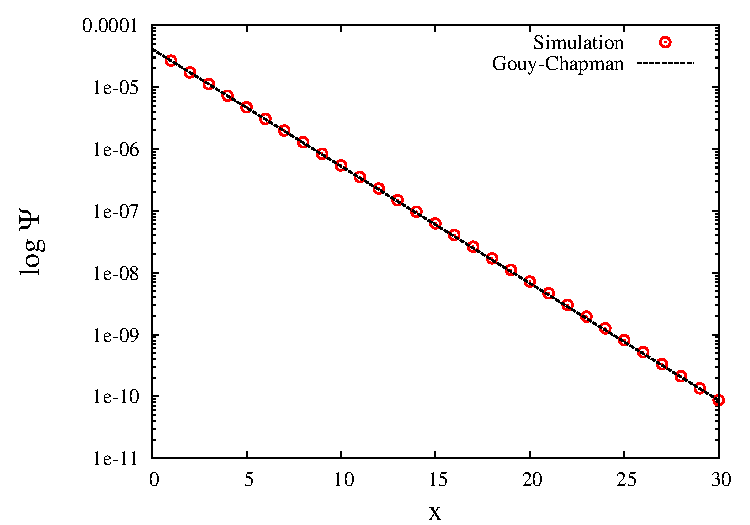
\includegraphics[width=0.495\textwidth]{./pics/test1.pdf}
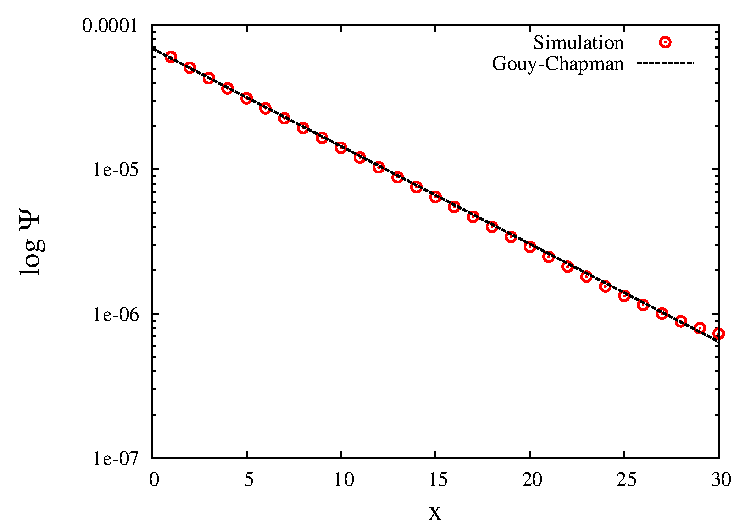
\includegraphics[width=0.495\textwidth]{./pics/test2.pdf}
\caption{Gouy-Chapman theory for electric double layers: The plots compare the simulation results for the electric potential with the analytical solution for $\rho_{0,\pm}=1\e{-2}$ (left) and $\rho_{0,\pm}=1\e{-3}$ (right).} 
\label{fig1} 
\end{figure}


\begin{equation}\label{gouychapman}
\Psi(x) = \Psi_D \exp(-\kappa\, x)
\end{equation}
with $\kappa$ as inverse Debye length 
\begin{equation}
\kappa = l_D^{-1} = \sqrt{8\pi\, l_B \, I}.
\end{equation}
The Bjerrum length $l_B$ is given by 
\begin{equation}
l_B = \frac{\beta\,e^2}{4\pi\,\varepsilon}
\end{equation} 

with $\beta^{-1}=k_B T$, $e$ as unit charge and $\varepsilon=\varepsilon_0\varepsilon_r$ 
as dielectric permittivity.
The parameter 

\begin{equation}
I = \frac{1}{2}\sum_k z_k^2\; \rho_{B,k}
\end{equation} 

is the ionic strength 
of the electrolyte with $z_k$ as valencies of species $k$
($z_\pm=\pm 1$ for simple symmetric electrolyte) and $\rho_{B,k}$ as 
bulk charge density of species $k$ far away from the wall.
The Stern potential $\Psi_D$ at the surface of the wall is related 
to the surface charge $\sigma$ via

\begin{eqnarray}
\Psi_D&=&\frac{2}{\beta \,e} \sinh^{-1}\left(-\sigma\,p\right)\\
\Psi_D&\simeq&\frac{2}{\beta \,e} \ln\left(-\sigma \, p + \sqrt{(\sigma\,p)^2+1}\right)\\
p &=& \frac{1}{\sqrt{8\, \varepsilon\, \beta^{-1} \,\rho_B}}.
\end{eqnarray}

The quantity $\rho_B=\rho_{B,+}=\rho_{B,-}$ is 
the average bulk charge density of the electrolyte.

We solved the Gouy-Chapman problem for a 
system consisting of $L_x \times L_y \times L_z=64\times4\times4$
lattice sites. Periodic boundary conditions were used at all sides 
and a no-flux boundary conditions was set at $L_x=1$ and $L_x=64$.

\begin{figure}[htpb]
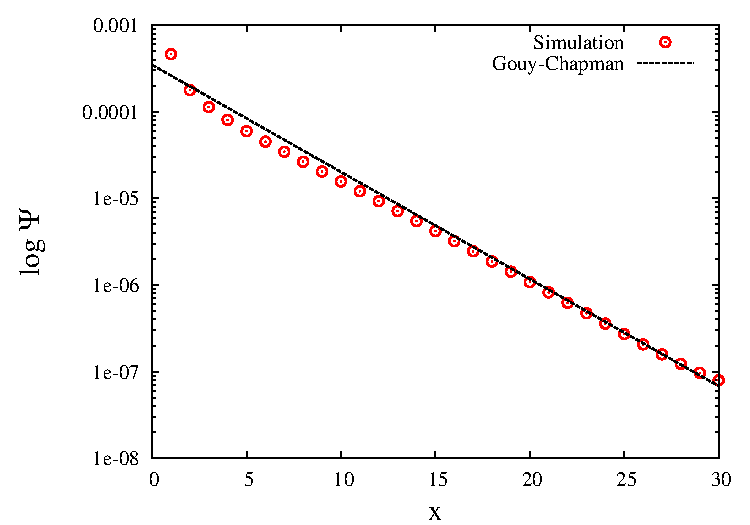
\includegraphics[width=0.495\textwidth]{./pics/test3.pdf}
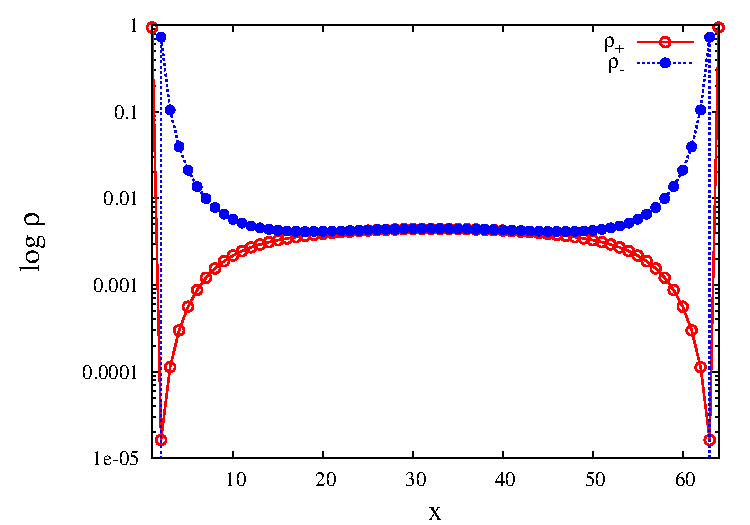
\includegraphics[width=0.495\textwidth]{./pics/test3-rho.pdf}
\caption{Nonlinear regime: For larger surface charges the solution deviates from the low-potential approximation Eq. \ref{gouychapman} to the Gouy-Chapman theory. The righthand picture shows the charge distribution across the gap.} 
\label{fig2} 
\end{figure}

 
The parameters were chosen as follows (all in simulation units):
unit charge $e=1$, temperature $k_B T=\beta^{-1}=3.333\e{-5}$, valency $z_{\pm}=\pm1$, 
dielectric permittivity $\varepsilon=3.3\e{3}$, diffusivities 
of the species $D_{\pm}=1\e{-2}$ and initial densities $\rho_{0,\pm}=1\e{-2}$.
The entire system was electro-neutral and had a Bjerrum length $l_B=0.723$.

At first we tested the linear case applying a small positive surface charge
$\sigma=3.125\e{-2}$, which led to bulk charge density $\rho_{B,+}=\rho_{B,-}=1.044\e{-2}$, 
Debye length $l_D=2.295$ and surface potential $\Psi_D=2.136\e{-5}$.
The potential was initialised with zero and had a value $\Psi_c=-2.364\e{-6}$ 
in the centre of the system after equilibration which we subtracted in the 
following analysis.

We reduced the initial density of the electrolyte to $\rho_{0,\pm}=1\e{-3}$,
which resulted in bulk charge densities  
$\rho_{B,+}=1.298\e{-3}, \rho_{B,-}=1.370\e{-3}$, 
Debye length $l_D=6.420$, surface potential $\Psi_D=5.451\e{-5}$
and centre potential $\Psi_c=-1.256\e{-5}$.
The comparison with the approximate solution Eq. \ref{gouychapman} is shown 
in Fig. \ref{fig1}.

For larger surface charges the low-potential assumption which led to Eq. \ref{gouychapman}
is no longer valid and the nonlinear nature of the Poisson-Boltzmann 
equation becomes evident.
Fig. \ref{fig2} shows the results for a surface charge $\sigma=9.375\e{-1}$
and electrolyte density $\rho_{0,\pm}=3\e{-3}$. We obtained for   
bulk charge densities $\rho_{B,+}=4.443\e{-3}$ and $\rho_{B,-}=4.461\e{-3}$, 
Debye length $l_D=3.514$, the surface potential $\Psi_D=2.267\e{-4}$
and the centre potential $\Psi_c=-3.395\e{-5}$. 

\subsubsection{Liquid-junction potential}

The liquid junction potential 
is a charge separation process that 
occurs when electrolytes with slightly different concentrations
whose species have different diffusivities are brought into contact.
Charges from the regions of higher concentration diffuse   
into the parts with lower concentration. Due to the difference 
in diffusivity they migrate at different speeds, leaving parts of
the system charged. This leads to a build-up of a potential
which balances the diffusive flux.

After the initial build-up phase the potential decreases slowly 
again until the charge concentration has become homogeneous throughout 
the system. Both timescales of emergence and decay of the potential
can be separated by chosing a sufficiently large system size.

This problem allowed us to verify the correct temporal 
behaviour of the Nernst-Planck equation solver by resolving the transient 
dynamics without having to account for advective terms.

\begin{figure}[h!t]
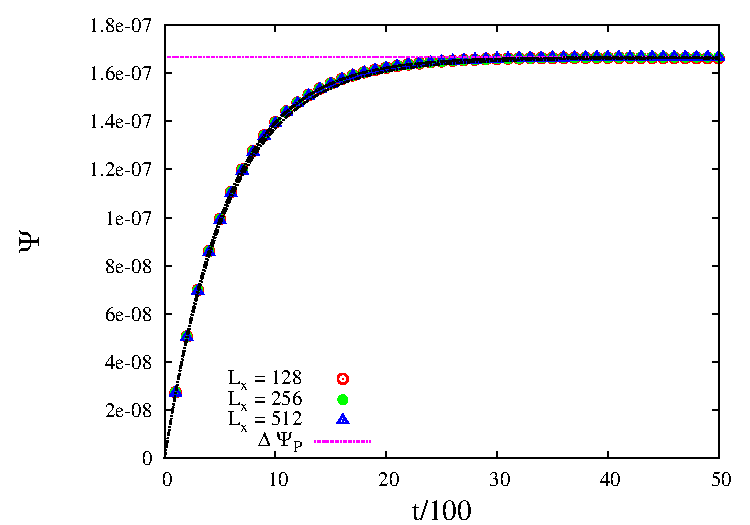
\includegraphics[width=0.495\textwidth]{./pics/test_lj_zoom1.pdf}
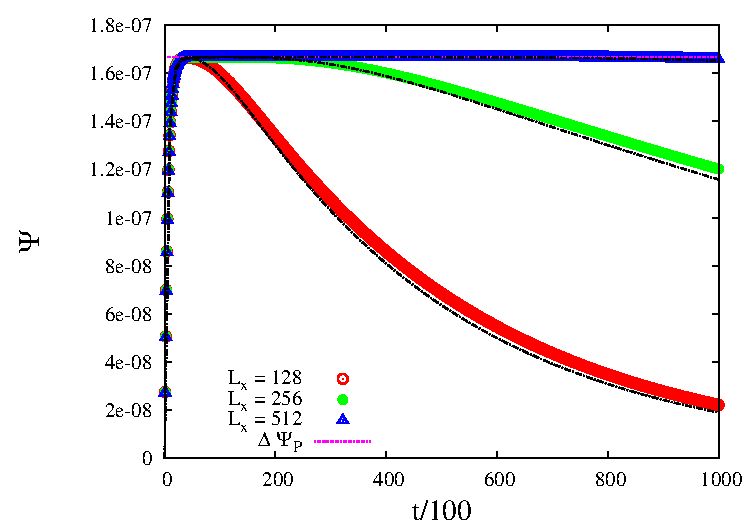
\includegraphics[width=0.495\textwidth]{./pics/test_lj_zoom3.pdf}
\caption{Time evolution of the liquid junction potential for $L_x=128$ (blue), $L_x=256$ (green) and $L_x=512$ (blue). The dashed black curves represent the approximate solution in the limit $l_D/L_x<<1$. Deviations can be seen which are presumably due
to the approximate nature of the analytical solution and the fact that we
have a different asymptotic flux close to the boundary - the theoretical 
analysis assumes no flux at a boundary which is infinitely far away from
the diffusive region.} 
\label{fig3} 
\end{figure}

For simplicity we considered systems of size 
$L_x\times L_y\times Lz=128\times4\times4$ and 
$L_x\times L_y\times Lz=256\times4\times4$ with
periodic boundary conditions at either end.
The two halfs were electroneutral and had ionic concentrations 
$\rho_{L,\pm}=\rho_{0,\pm} + \delta\rho$ and 
$\rho_{R,\pm}=\rho_{0,\pm} - \delta\rho$ 
with $\rho_{0,\pm}=1\e{-2}$ and $\delta\rho = 0.01$.

The potential difference between both sides during the build-up 
obeys approximately

\begin{equation}
\Delta\Psi(t)\simeq\Delta\Psi_P \left\{1-\exp\left(-\frac{t}{\tau_e}\right)\right\}\\
\end{equation}

with 

\begin{equation}
\Delta\Psi_P=\frac{(D_+ D_-)}{\beta e (D_+ + D_-)} \frac{\delta\rho}{\rho_0}\\ 
\end{equation}

as saturation value of the potential difference.
The saturation time scale is given by

\begin{equation}
\tau_e=\frac{\varepsilon}{\beta \, e^2 (D_+ + D_-) \rho_0}.
\end{equation}

\begin{figure}[htpb]
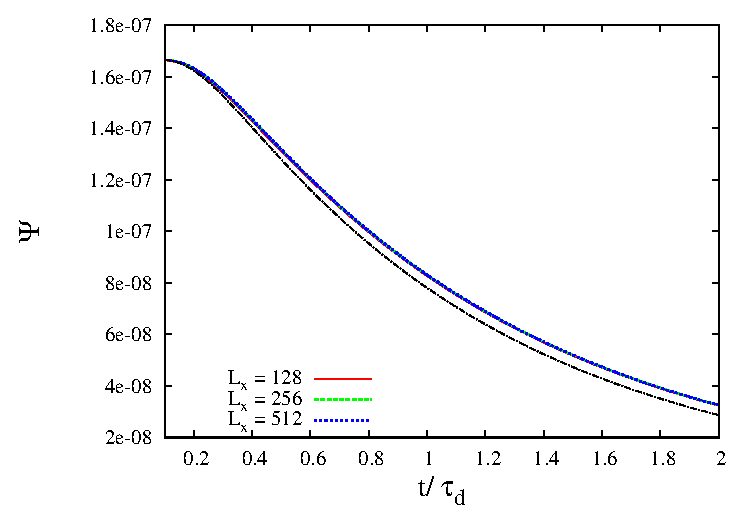
\includegraphics[width=0.9\textwidth]{./pics/test_lj_decay1.pdf}
\caption{Rescaled plot of the decay: Times have been Time evolution of the liquid junction potential for $L_x=128$ (blue), $L_x=256$ (green) and $L_x=512$ (blue). The dashed black curves represent the approximate solution in the limit $l_D/L_x<<1$. Deviations can be seen which are due
to the approximate nature of the analytical solution and the diffusive fluxes close to the boundary.} 
\label{fig4} 
\end{figure}

A more exact solution can be derived in the limit $l_D/L_x<<1, N\to\infty$: 
 
\begin{eqnarray}
\Delta\Psi(t)&=&\Delta\Psi_P \left\{1-\exp\left(-\frac{t}{\tau_e}\right)\right\}\frac{4}{\pi}\left\{\sum_{m=1}^N \frac{\sin^3(m\pi/2)}{m} \exp\left(-\frac{ m^2\, t}{\tau_d}\right)\right\}\\
\tau_d&=&\frac{L^2}{2\pi^2 (D_+ + D_-)}.\label{taud}
\end{eqnarray}

It contains as well the dependence on the decay timescale $\tau_d$.
Only odd indices $m$ contribute to the sum:
 
\begin{eqnarray}
\sum_{m=1}^N \frac{\sin^3(m\pi/2)}{m} \exp\left(-\frac{m^2\, t}{\tau_d}\right)&=&\nonumber\\
&&\hspace*{-4cm} \exp\left(-\frac{t}{\tau_d}\right)-\frac{1}{3} \exp\left(-\frac{9 t}{\tau_d}\right)+\frac{1}{5}\exp\left(-\frac{25t}{\tau_d}\right)-\frac{1}{9}\exp\left(-\frac{81 t}{\tau_d}\right)+\ldots
\end{eqnarray}

A complete discussion of the solution can be found in \cite{Mafe}. 
There, the upper limit of significant modes has been also estimated as $N_{max} = L/\pi l_D$.
Note the factor 2 difference between Eq. \ref{taud} and the corresponding expression in \cite{Mafe}.

The following parameters were used:
dielectric permittivity $\epsilon=3.3\e{3}$, temperature $\beta^{-1}=3.333\e{-5}$, unit charge $e=1$, valency $z_\pm=\pm1$, diffusivities $D_+=0.0125$ and $D_-=0.0075$.
We obtained
$\Delta\Psi_P=1.6667\e{-7}$, $\tau_e=550$, $\tau_d=41501.2\, (L_x=128)$, $\tau_d=166004.6\, (L_x=256)$ and $\tau_d=664018.5 (L_x=512)$.
The results for the potential difference over time are shown in Fig. \ref{fig3}.

Fig. \ref{fig4} shows results with times rescaled to the decay 
time scale $\tau_d$ (cf. Eq. \ref{taud}). Obviously the 
deviations we observe are not due to the limited system size 
and have a more systematic origin. 

The curves coincide if 
the theoretic limit for $\tau_d$ is rescaled by a factor $1.067$,
suggesting the effective system length for this sort of setup is
actually about 3\% larger than the numerical value.

A reason for this might be the approximate nature of the analytical solution 
and the fact that it was gained
for an infinitely large system with constant charge concentrations,
vanishing currents at both ends and finite diffusive zone of size $L_x$.
In our situation the entire system is within the diffusive zone.
This may lead to smaller effective diffusivities or larger effective
system sizes.
Interestingly, all runs with solid walls at both ends resulted in 
oscillatory behaviour and an effective system size of $2L_x$.


\subsubsection{Electroosmotic Flow}

To test the implementation with all couplings to external and 
internal forces we consider a forced charged fluid in a slit
of size $L_z$. An electrostatic field $E_{||}$ is allied
parallel to the walls. The entire system is electroneutral with 
each wall having the surface charge density $\sigma$ 
and compensationg counterions with total charge $2 \sigma A_{wall}$
in the fluid.

In equilibrium the charge density at a distance $x$ from the wall obeys

\begin{equation}
\rho(x)=\frac{\rho_0}{\cos^2(K\,x)}
\end{equation}

with 

\begin{equation}
\rho_0=K^2/2\pi l_B
\end{equation}

and 

\begin{eqnarray}
K \,L_x \tan\left(\frac{K\, L_x}{2}\right)&=&\pi\, l_B\, L_x\, 2\sigma\label{kex} \\
K \,L_x&\simeq&\sqrt{4\pi \,l_B\,L_x\,2\sigma}\label{klin}.
\end{eqnarray}


The liniarised version Eq. \ref{klin} has only a limited range of applicabilty.
We solved Eq. \ref{kex} numerically and found solutions 
$K=0.01959\; (\sigma=0.003125)$ and $K=0.03311\; (\sigma=0.00125)$, 
which is reasonably far away from the 
theoretical limit $K_{max}=\pi/L_x$ set by the tangent. 

Note the factor 2 difference on the lhs of Eq. \ref{kex} with respect 
to \cite{Capuani, Rotenberg}. There is also a factor $L_x$ missing on 
the rhs of Eq. \ref{klin}.

The steady state velocity of the fluid can be derived from the 
force balance of the gradient of the stresses and the electrostatic
forces:

\begin{eqnarray}
v_y(x)&=&\hat{v} \ln\left(\frac{\cos(K\,x)}{\cos(K\,L_x/2)}\right)\label{vy}\\
\hat{v}&=&\frac{e \,E_{||}\rho_o}{\eta\, K^2}=\frac{e \,E_{||}}{2\pi\eta l_B}\label{vhat}
\end{eqnarray}

The result for two different charge densities is shown in Fig. \ref{fig6}.
The accuracy is acceptable with deviations for high surface 
charged potentially being caused by the chosen discretisation or 
by the numerical solution of Eq. \ref{kex} approaching the limit 
of $\pi/L_z\simeq0.049$.  

\begin{figure}[htpb]
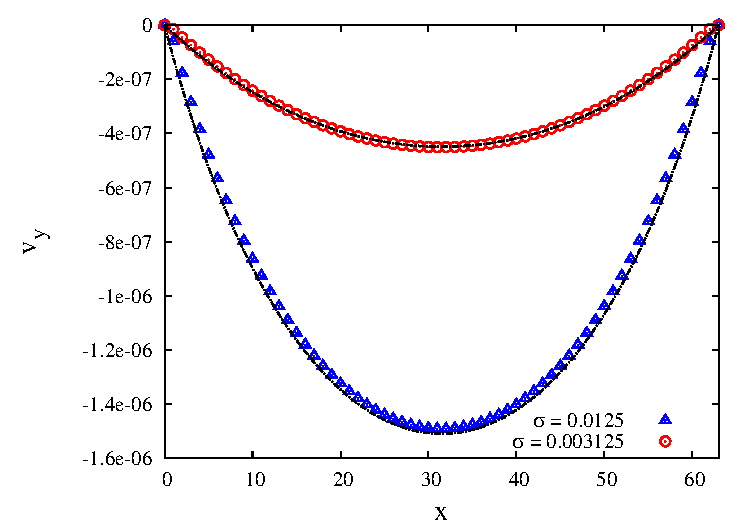
\includegraphics[width=0.9\textwidth]{./pics/test_eo.pdf}
\caption{Steady state flow profile across a slit of width $L_x=63$ for an applied field of magnitude $e \beta E L_x=1.89$ for two different charge densities $\sigma=0.003125$ (red) and $\sigma=0.0125$ (blue), Bjerrum length $l_B=0.7234$, viscosity $\eta=0.1$ and unit charge $e=1$. The dashed black lines correspond to theoretical prediction according to Eqs. \ref{vy} and \ref{vhat}.} 
\label{fig6} 
\end{figure}

\subsubsection{Debye-H\"uckel Theory}

We have tested the implementation for a single fixed
colloid and compared the result with Debye-H\"uckel theory. A result
is shown in Fig.~\ref{fig7}.
We used the following parametrisation:

$L_x \times L_y \times L_z=64\times64\times64$,
$D_+=D_-=0.01$,
$e=1$, 
$z_{\pm}=1$,
$\beta^{-1}=3.333\e{-5}$,
$\varepsilon=3.3\e{3}$,
$l_B=0.723$.

For a central and fixed colloid of radius $R_c=7.5$ carrying a positive unit charge
$q_{c,+}=1.0, q_{c,-}=0$ we obtained 
$\rho_{c,+}=5.58\e{-4}$,
$\rho_{el}=\rho_{B,\pm}=1\e{-2}$, 
$\Psi_D=8.836\e{-7}$ for $2\,R_c=16$.

For a higher larger positive charge $q_{c,+}=4.0$ we got
$\rho_{c,+}=2.23\e{-3}$
$\rho_{el}=\rho_{B,\pm}=5\e{-3}$ 
$\Psi_D=4.993\e{-6}$ for $2\,R_c=16$.

\begin{figure}[htpb]
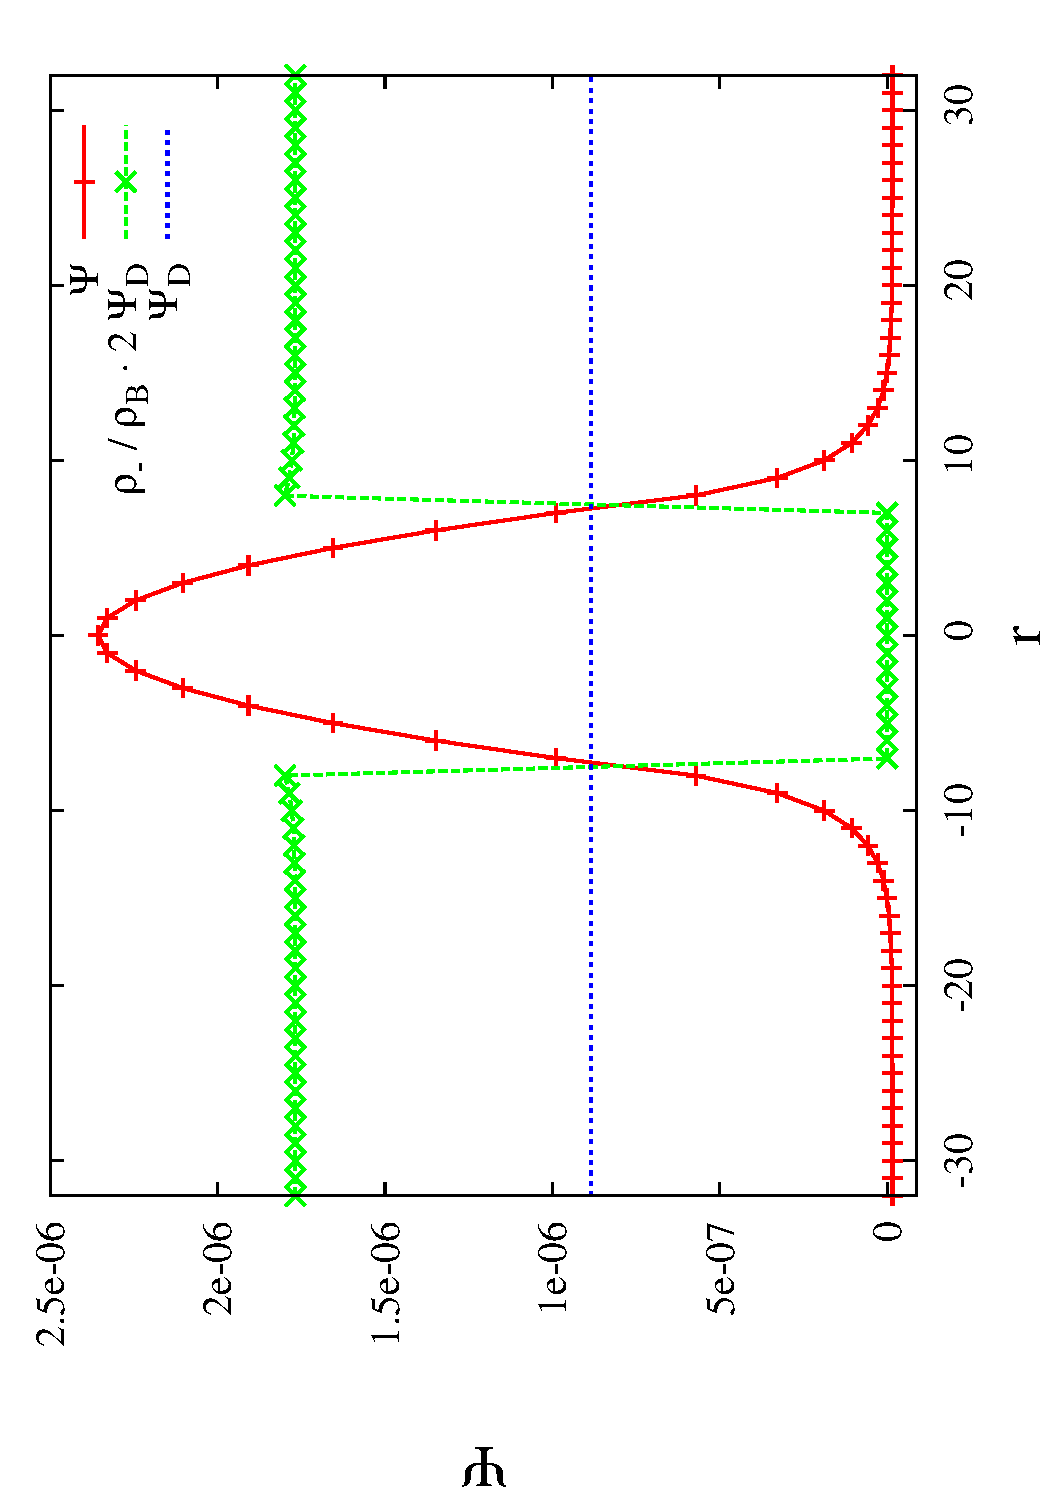
\includegraphics[angle=-90,width=0.9\textwidth]{./pics/test_dh1.pdf}\\
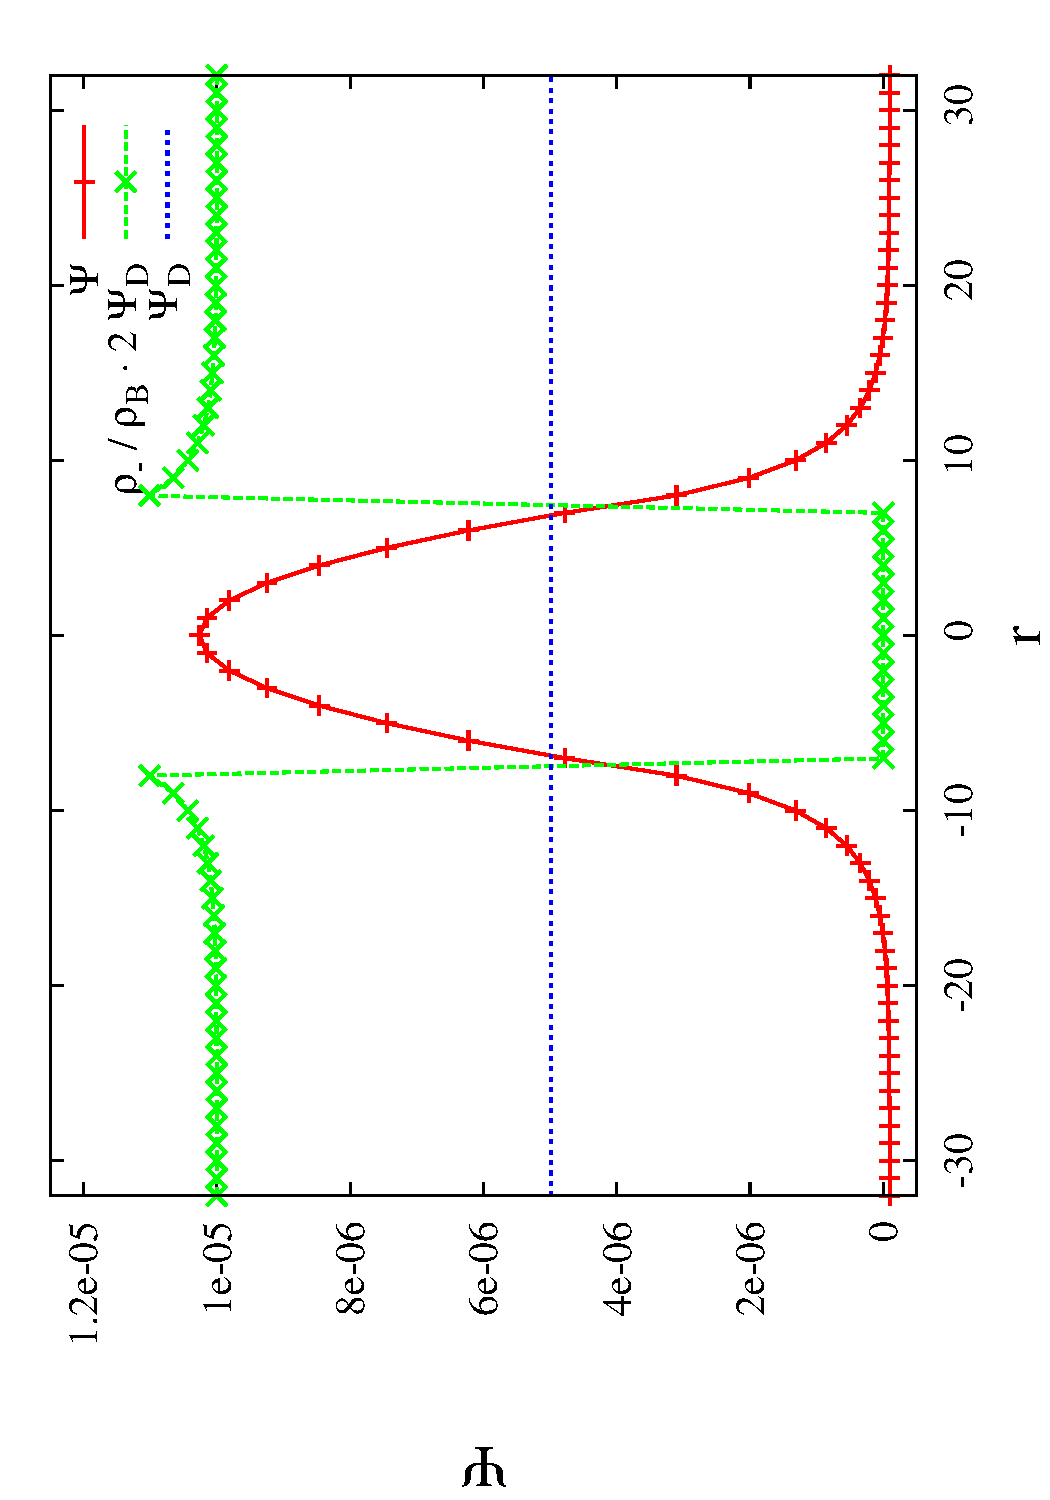
\includegraphics[angle=-90,width=0.9\textwidth]{./pics/test_dh2.pdf}
\caption{Debye-H\"uckel theory for positively charged colloid: the picture
shows a cut through the center of a single colloid in a peridoic system.
The potential is shown in red, the Stern potential in blue, and the negative 
charge density in green. The colloid is in the center.}
\label{fig7}
\end{figure}
\clearpage
